% =====================================================================
%  PROMETHEUS CITADEL — team brief
%  Compile with pdfLaTeX. Run twice.
% =====================================================================
\documentclass[11pt]{article}

\usepackage[T1]{fontenc}
\usepackage[utf8]{inputenc}
\usepackage{lmodern}
\usepackage{microtype}
\usepackage[margin=0.85in,headheight=15pt,footskip=26pt]{geometry}
\usepackage{parskip}
\usepackage{enumitem}
\usepackage{booktabs}
\usepackage{tabularx}
\usepackage{array}
\usepackage[table]{xcolor}
\usepackage{tikz}
\usetikzlibrary{arrows.meta,positioning,shapes.geometric,fit,calc}
\usepackage[most]{tcolorbox}
\usepackage{adjustbox}
\usepackage{titlesec}
\usepackage{fancyhdr}
\usepackage{hyperref}

% ---------- the model, named in exactly one place ----------
\newcommand{\themodel}{GPT-4o-mini}

% ---------- the game's palette ----------
\definecolor{PageBG}{HTML}{0B0710}
\definecolor{Panel}{HTML}{1C1119}
\definecolor{Cream}{HTML}{F2E8DC}
\definecolor{Coral}{HTML}{E08D6D}
\definecolor{Gold}{HTML}{FFD87A}
\definecolor{Teal}{HTML}{7FE9D6}
\definecolor{Muted}{HTML}{9B8BA0}
\definecolor{Deep}{HTML}{140C13}   % a shade between page and panel, for rules

\usepackage{graphicx}
\graphicspath{{shots/}}
% a screenshot in the game frame: coral hairline, rounded, with a muted caption
\newcommand{\shot}[2]{%
  \begin{center}
  \begin{tcolorbox}[enhanced,colback=Panel,colframe=Coral,boxrule=0.6pt,
      arc=1.4mm,left=0.6mm,right=0.6mm,top=0.6mm,bottom=0.6mm,width=\linewidth]
    \includegraphics[width=\linewidth]{#1}%
  \end{tcolorbox}%
  \vspace{-0.2em}{\footnotesize\itshape\color{Muted}#2}
  \end{center}}

\hypersetup{
  colorlinks=true, linkcolor=Gold, urlcolor=Teal, citecolor=Gold,
  pdftitle={Prometheus Citadel: a team brief},
  pdfauthor={Gokulakrishnan, Padmanabha, Taha, Naimah, Amarah}
}

\setlist[itemize]{leftmargin=1.15em,itemsep=0.25em,topsep=0.3em,parsep=0pt}
\setlist[enumerate]{leftmargin=1.4em,itemsep=0.25em,topsep=0.3em,parsep=0pt}

% ---------- headings ----------
\titleformat{\section}
  {\sffamily\Large\bfseries\color{Gold}}{\thesection}{0.6em}{}
  [\vspace{0.35em}{\color{Coral}\titlerule[1pt]}]
\titleformat{\subsection}
  {\sffamily\large\bfseries\color{Coral}}{\thesubsection}{0.5em}{}
\titlespacing*{\section}{0pt}{1.6em}{1.0em}
\titlespacing*{\subsection}{0pt}{1.0em}{0.35em}

% ---------- running head ----------
\pagestyle{fancy}
\fancyhf{}
\lhead{\sffamily\small\bfseries\color{Coral}PROMETHEUS CITADEL}
\rhead{\sffamily\small\color{Muted}team brief}
\cfoot{\sffamily\small\color{Muted}\thepage}
\renewcommand{\headrule}{\color{Muted}\hrule height 0.4pt \vspace{2pt}}
\renewcommand{\footrulewidth}{0pt}

\fancypagestyle{plainhead}{\fancyhf{}\cfoot{\sffamily\small\color{Muted}\thepage}%
  \renewcommand{\headrule}{}}

% ---------- boxes, all readable on the dark page ----------
\tcbset{
  briefbase/.style={
    enhanced, breakable, boxrule=0.9pt, arc=2.2mm,
    left=3.4mm, right=3.4mm, top=2.8mm, bottom=2.8mm,
    colback=Panel, coltext=Cream,
    fontupper=\linespread{1.06}\selectfont
  }
}
\newtcolorbox{snarebox}[1][]{briefbase, colframe=Gold, #1}
\newtcolorbox{shieldbox}[1][]{briefbase, colframe=Teal, #1}
\newtcolorbox{gamebox}[1][]{briefbase, colframe=Coral, #1}
\newtcolorbox{quietbox}[1][]{briefbase, colframe=Muted, #1}

% ---------- table rules that survive a dark page ----------
\arrayrulecolor{Muted}
\newcolumntype{L}[1]{>{\raggedright\arraybackslash}p{#1}}
% NOTE: never put \color in the preamble of a p/L/X column. The whatsit it
% leaves at the head of the cell drops the whole cell half a line below its
% neighbour. Use \textcolor inside the cell instead.

% ---------- diagram styles, same palette ----------
\tikzset{
  every node/.append style={text=Cream},
  box/.style={draw=Muted, line width=0.9pt, rounded corners=1.6mm, fill=Panel,
              align=center, minimum height=11mm, text width=29mm,
              inner sep=2.2mm, font=\sffamily\small},
  hot/.style={box, draw=Coral},
  gld/.style={box, draw=Gold},
  cool/.style={box, draw=Teal},
  arrow/.style={-{Latex[length=2.4mm,width=2.0mm]}, line width=0.9pt, draw=Muted},
  arrowhot/.style={arrow, draw=Coral},
  arrowcool/.style={arrow, draw=Teal},
  tag/.style={font=\sffamily\small, text=Muted, inner sep=1pt},
}

\newcommand{\kicker}[1]{{\sffamily\footnotesize\bfseries\color{Muted}#1\par\vspace{0.15em}}}
\newcommand{\snare}[1]{\textcolor{Gold}{\textbf{#1}}}

\begin{document}
\pagecolor{PageBG}
\color{Cream}

% =====================================================================
% TITLE
% =====================================================================
\begin{titlepage}
\thispagestyle{empty}
\vspace*{0.9cm}

{\sffamily\footnotesize\bfseries\color{Coral}A MONSTER GAME THAT HAPPENS TO TEACH\par}
\vspace{0.45cm}
{\sffamily\fontsize{44}{46}\selectfont\bfseries\color{Gold}PROMETHEUS\\CITADEL\par}
\vspace{0.55cm}
{\Large\color{Cream}Five monsters hold a citadel. Each one feeds on a
different way of being wrong.\par}

\vspace{1.1cm}
\begin{snarebox}
\centering\large
Every wrong answer in the game carries a \snare{snare}:\\[0.3em]
the exact wrong idea that makes that answer feel right.\\[0.55em]
The monsters live on snares.\\[0.3em]
You win by proving yours no longer works on you.
\end{snarebox}

\vspace{0.9cm}
{\color{Muted}\hrule height 0.6pt}
\vspace{0.7cm}

\begin{tabularx}{\textwidth}{@{}>{\sffamily\bfseries\color{Coral}}l X@{}}
What it is & An offline game for Ontario's Grade 9 EQAO mathematics\\
           & assessment\\[0.4em]
Where it runs & A Streamlit web app, deployed online. \themodel\ is called
               over the network via the OpenAI API\\[0.4em]
Event & Originally built for Build with AI --- Gemma Hackathon, GDG Windsor\\[0.4em]
Track & \emph{Originally} Edge / On-Device --- the project has since moved
        from a locally-served model to a cloud API, so this track claim
        needs re-confirming with organisers before submission\\[0.4em]
Team & Gokulakrishnan, Padmanabha, Taha, Naimah, Amarah\\
\end{tabularx}

\vspace{1.4cm}
{\centering
{\sffamily\small\bfseries\color{Coral}FRACTIS $\cdot$ EQUAZOR $\cdot$ STATIQ
$\cdot$ POLYGOR $\cdot$ LEDGERLING\par}
\vspace{0.35em}
{\small\color{Muted}and, above all five, the Collector\par}
\par}

\vfill
{\color{Muted}\hrule height 0.4pt}
\vspace{0.5em}
{\small\color{Muted}No account needed. An internet connection is required
during play: quiz answers and typed reasoning are sent to OpenAI's servers as
part of each \themodel\ call.\par}
\end{titlepage}

% =====================================================================
\section{Enter the citadel}

Every Grade 9 student in Ontario sits EQAO, the province's mathematics
assessment, written once and marked province-wide. Around Windsor--Essex it is
a date the whole house knows about. What is on
offer is sixty dollars an hour for someone to sit beside them, or an app that
puts a red X next to the answer and moves on.

The red X is the problem. A wrong answer in maths is almost never random. Ask a
fourteen-year-old for $2/3 + 1/4$ and watch for $3/7$. Tops with tops, bottoms
with bottoms. Tidy, symmetric, and wrong. Marking it wrong teaches nothing,
because the student who wrote $3/7$ already believed $3/7$. That is not
carelessness. It is a rule, applied faithfully. It is just the wrong rule.

We call each one a \snare{snare}. A snare has a name, and once you can name it
you can hunt it.

\begin{snarebox}
\textbf{The rule of the game.} A monster sets a snare. You get caught. You beat
the snare by answering fresh questions right \emph{and} showing the path you
took. Then the monster has nothing left to eat.
\end{snarebox}

\shot{citadel.png}{The citadel. Five monsters, one on each platform, and the
sealed keep behind them. Click one to face it.}

Five monsters guard the citadel, one for each strand EQAO assesses.

\vspace{0.4em}
\begin{center}
\begin{tabularx}{0.97\textwidth}{@{}>{\sffamily\bfseries}l l X@{}}
\toprule
\textcolor{Gold}{\sffamily MONSTER} & \textcolor{Gold}{\sffamily GUARDS} &
\textcolor{Gold}{\sffamily LIVES ON}\\
\midrule
\textcolor{Coral}{Fractis} & Number & Fractions added straight across\\
\textcolor{Coral}{Equazor} & Algebra & A sign that slips crossing the equals\\
\textcolor{Coral}{Statiq} & Data & Mean and median blurred together\\
\textcolor{Coral}{Polygor} & Geometry \& Measurement & A formula that is almost right\\
\textcolor{Coral}{Ledgerling} & Financial Literacy & Money and time, quietly mixed up\\
\bottomrule
\end{tabularx}
\end{center}
\vspace{0.4em}

Pick a monster and the camera flies in to its torch-lit hall, where it taunts
you and then puts five questions to you --- real EQAO-style questions, pulled
from the game's vault of verified ones. This first battle is a diagnosis
dressed up as a fight: the game is not trying to teach you yet, it is watching
which snares catch you. Every wrong option on every question already has a snare
written beside it, put there when the question was written. So when you pick a
wrong answer, the game does not have to guess what went wrong inside your head.
It reads the label.

\vspace{0.5em}
\begin{center}
\begin{adjustbox}{max width=\textwidth}

\begin{tikzpicture}[node distance=8mm]
  \node[hot] (choose) {Pick a monster};
  \node[box, right=of choose] (fight) {Five questions from the vault};
  \node[gld, right=of fight] (snare) {The snare that caught you most};
  \node[cool, right=of snare] (train) {Training, until it stops working};
  \node[hot, right=of train] (back) {Back to the hall};
  \draw[arrow] (choose)--(fight);
  \draw[arrow] (fight)--(snare);
  \draw[arrowhot] (snare)--(train);
  \draw[arrowcool] (train)--(back);
\end{tikzpicture}
\end{adjustbox}
\end{center}

% =====================================================================
\section{One battle with Ledgerling}

Ledgerling guards Financial Literacy and charges interest on every mistake.
Here is one of its five questions, exactly as it sits in the vault.

\begin{snarebox}
\textbf{FIN-Q1} \quad {\small\color{Muted}Financial Literacy $\cdot$ budgeting
and saving}

\medskip
Priya has a part-time job in Barrie and earns \$800 each month. She saves 3\%
of her earnings every month. How much money will she have saved in total after
6 months?

\medskip
{\centering A. \$14,400.00 \quad B. \$4,656.00 \quad
\textcolor{Teal}{C. \$144.00} \quad D. \$24.00\par}
\end{snarebox}

The answer is C, and the vault carries the working with it:
\[
  0.03 \times 800 = \$24 \text{ each month},\qquad 6 \times 24 = \$144 .
\]

Say you pick D. You are not lost --- you found \$24 correctly and then stopped.
That option is labelled \snare{Time-period mishandling}, and Ledgerling eats
well tonight.

The other two wrong answers are different snares on the same question. A is
\snare{Percent--decimal conversion error}: multiply by 3 instead of 0.03 and
you get \$2{,}400 a month. B is \snare{Wrong quantity reported}: \$4{,}656 is
the money Priya did \emph{not} save. Three players can miss this one question
for three different reasons and get three different evenings.

Across the five questions of the battle, the game keeps a tally. The snare that
fed the monster most is the one it goes after first.

\vspace{0.5em}
\begin{center}
\begin{adjustbox}{max width=\textwidth}
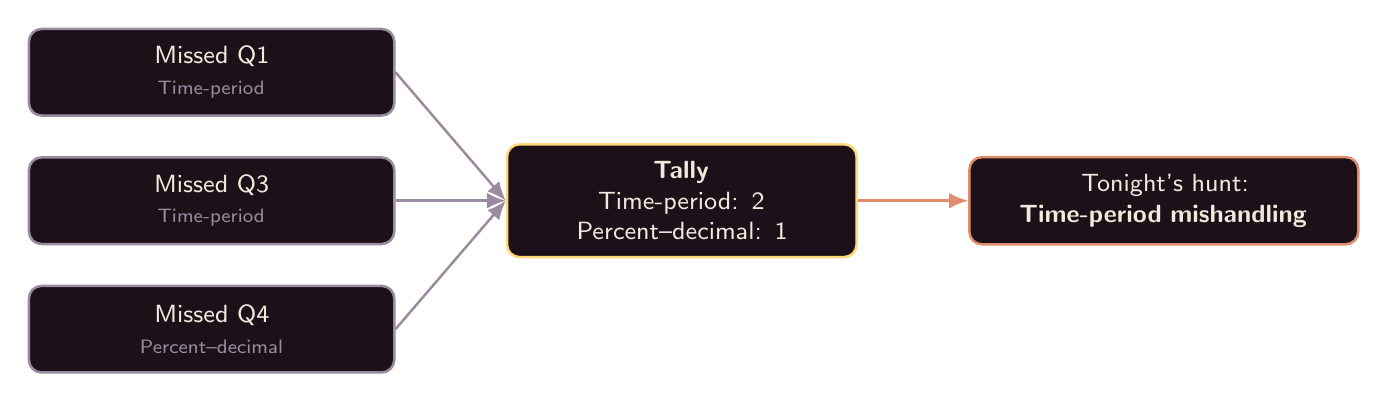
\begin{tikzpicture}[node distance=5mm and 14mm]
  \node[box, text width=42mm] (q1) {Missed Q1\\{\scriptsize\color{Muted}Time-period}};
  \node[box, below=of q1, text width=42mm] (q2) {Missed Q3\\{\scriptsize\color{Muted}Time-period}};
  \node[box, below=of q2, text width=42mm] (q3) {Missed Q4\\{\scriptsize\color{Muted}Percent--decimal}};
  \node[gld, right=of q2, text width=40mm] (tally) {\textbf{Tally}\\Time-period: 2\\Percent--decimal: 1};
  \node[hot, right=of tally, text width=45mm] (first) {Tonight's hunt:\\\textbf{Time-period mishandling}};
  \draw[arrow] (q1.east)--(tally.west);
  \draw[arrow] (q2.east)--(tally.west);
  \draw[arrow] (q3.east)--(tally.west);
  \draw[arrowhot] (tally)--(first);
\end{tikzpicture}
\end{adjustbox}
\end{center}

Nothing in that diagram is a judgement call. The labels come from the vault,
the counting is arithmetic, and the biggest number wins. \themodel\ has not
been asked anything yet.

% =====================================================================
\section{How you beat a snare}

Now the game switches from testing to teaching, and it works one snare at a
time --- the one that caught you most. A \emph{check question} is just a fresh
question of the same kind you got wrong: one you have not seen, so you cannot
have memorised the answer. But getting it right is only half of what the game
wants. Under every check question is a single line where you type, in your own
words, \emph{how} you got there. That line is the whole point. Anyone can
stumble onto the right letter; the game is trying to find out whether you
actually understand, and the only way to tell the difference is to hear you
explain it. One lucky answer proves nothing, so one lucky answer is not the bar.
The loop below runs until you clear the bar or a safety cap stops it.

\vspace{0.5em}
\begin{center}
\begin{adjustbox}{max width=\textwidth}
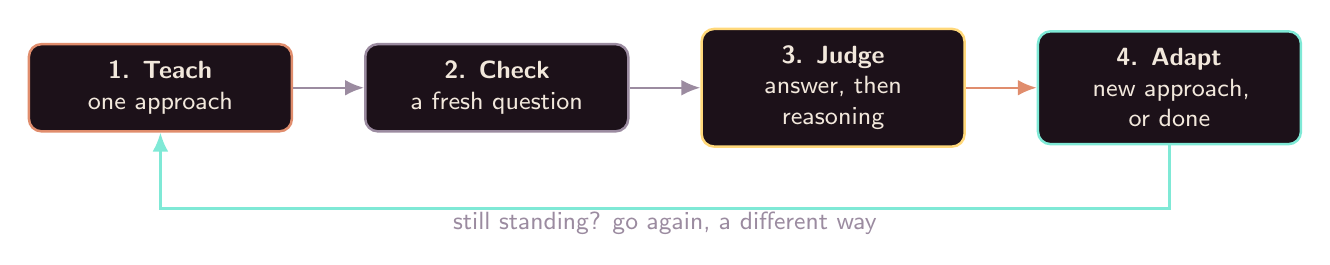
\begin{tikzpicture}[node distance=9mm]
  \node[hot] (teach) {\textbf{1. Teach}\\one approach};
  \node[box, right=of teach] (check) {\textbf{2. Check}\\a fresh question};
  \node[gld, right=of check] (judge) {\textbf{3. Judge}\\answer, then reasoning};
  \node[cool, right=of judge] (adapt) {\textbf{4. Adapt}\\new approach, or done};
  \draw[arrow] (teach)--(check);
  \draw[arrow] (check)--(judge);
  \draw[arrowhot] (judge)--(adapt);
  \draw[arrowcool] (adapt.south) -- ++(0,-8mm) -| (teach.south)
    node[tag, pos=0.25, below] {still standing? go again, a different way};
\end{tikzpicture}
\end{adjustbox}
\end{center}

\subsection{Four ways to explain, and no fifth}

If one explanation does not land, the game does not repeat it louder. It
changes the approach. There are exactly four, fixed in the code, and they are
tried in this order unless \themodel\ argues for a different one.

\vspace{0.3em}
\begin{center}
\begin{tabularx}{0.97\textwidth}{@{}>{\sffamily\bfseries}L{34mm} X@{}}
\toprule
\textcolor{Coral}{Direct correction} & Name the snare plainly --- ``you might think\ldots\ but
actually\ldots'' --- state the right rule in two or three sentences, then work
one example all the way through.\\
\addlinespace[0.3em]
\textcolor{Coral}{Visual walkthrough} & A concrete model walked through one step at a time: a
number line, an area model, groups of objects, a table. The point is to make you
see why it works, instead of handing you another rule to remember.\\
\addlinespace[0.3em]
\textcolor{Coral}{Side-by-side contrast} & The wrong method and the right method on the same
problem, line against line, with a finger on the exact step where they split.\\
\addlinespace[0.3em]
\textcolor{Coral}{Real-world analogy} & Money, pizza slices, game scores. Build the everyday
version first, then map it back onto the maths.\\
\bottomrule
\end{tabularx}
\end{center}

\vspace{0.3em}
When you get a check question wrong, \themodel\ reads what you typed and picks
which of the \emph{remaining} approaches to try next, and says why in one
sentence you can see. It cannot invent a fifth approach, cannot repeat one it
has already used, and cannot leave the ladder. If its answer does not name a
real approach, the code just takes the next rung and says so.

\subsection{The bar, and the three ways a night ends}

\begin{center}
\begin{adjustbox}{max width=\textwidth}
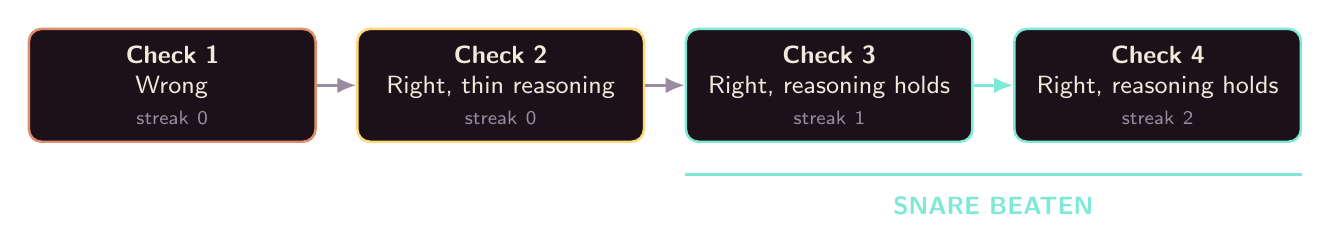
\begin{tikzpicture}[node distance=5mm]
  \node[hot, text width=32mm] (a) {\textbf{Check 1}\\Wrong\\{\scriptsize\color{Muted}streak 0}};
  \node[gld, right=of a, text width=32mm] (b) {\textbf{Check 2}\\Right, thin reasoning\\{\scriptsize\color{Muted}streak 0}};
  \node[cool, right=of b, text width=32mm] (c) {\textbf{Check 3}\\Right, reasoning holds\\{\scriptsize\color{Muted}streak 1}};
  \node[cool, right=of c, text width=32mm] (d) {\textbf{Check 4}\\Right, reasoning holds\\{\scriptsize\color{Muted}streak 2}};
  \draw[arrow] (a)--(b); \draw[arrow] (b)--(c); \draw[arrowcool] (c)--(d);
  \draw[line width=1.2pt, Teal] ([yshift=-4mm]c.south west)--([yshift=-4mm]d.south east)
    node[midway, below=1.5mm, font=\sffamily\small\bfseries, text=Teal]{SNARE BEATEN};
\end{tikzpicture}
\end{adjustbox}
\end{center}

\vspace{0.2em}
The bar is \textbf{two fresh questions right in a row}, with reasoning that
holds up. The reasoning box under each answer is optional and the submit button
never waits on it --- but when you do write something, it counts:

\begin{itemize}
  \item Right answer, reasoning that shows you understand: the streak goes up.
  \item Right answer, thin or circular reasoning: the streak stays where it is.
        You are not punished, but you have not shown anything yet.
  \item Right answer, reasoning that still contains the snare: the streak goes
        back to zero. You got there for the old wrong reason.
  \item Wrong answer: streak to zero, and a different approach next.
\end{itemize}

Three caps end the night, and all three are plain code: \textbf{four} check
questions, \textbf{twelve} model calls, or a ladder with no rungs left. When
one of them trips, the game stops and says which one. It does not drill you
into the ground, and it does not pretend.

\begin{quietbox}
\textbf{A fresh question is fresh, but it is not random.} Every follow-up is
modelled on the exact question you just got wrong, and stays on that same
topic. Not merely the same part of the course --- slope from two points and the
distributive property are both Algebra, and a player who could not solve the
equation is not helped by coordinate geometry. If the vault has nothing left on
that exact topic, the game would rather write a new question than hand you the
wrong one.
\end{quietbox}

% =====================================================================
\section{What the vault holds}

\begin{itemize}
  \item \textbf{55 questions} across the five parts of the course: Number,
        Algebra, Financial Literacy, Geometry \& Measurement, Data. The bank
        was audited against the published Grade 9 expectations and against what the
        EQAO assessment actually covers.
  \item \textbf{A worked solution on every single one.} That is what lets
        \themodel\ teach without being allowed to calculate.
  \item \textbf{A snare on every wrong option} --- 165 of them --- naming the
        faulty thinking that produces exactly that answer.
  \item \textbf{A balanced key}, 14/14/14/13 across A, B, C and D.
  \item \textbf{A topic on every question}, and the topic is a hard filter when
        the game hunts for your next one, not a preference.
\end{itemize}

Finding a follow-up is a tag lookup, not a search: the vault knows that NUM-6
and NUM-6b are the same idea at two depths, and it will take a sibling before
it takes a stranger. If nothing on your topic is left, it returns nothing ---
and returning nothing is a real answer. The game then writes a question under
audit, or stops and says the vault is out. Either beats practising the wrong
thing.

% =====================================================================
\section{Ten jobs for \themodel, one door}

\themodel\ is not decoration on top of a quiz app. Take it out and there is no
lesson, no judgement, no direction, and no letter home --- just a marked test.
Here is every job it does.

\newcommand{\job}[2]{\vspace{0.55em}\noindent{\sffamily\bfseries\color{Gold}#1.}\quad #2\par}

\job{1 -- It writes the lesson}{Not a template with your numbers dropped in. It
writes the teaching itself, in the style of whichever approach is currently
being tried. What it does not get is freedom with the maths: the verified
working from the vault rides inside the prompt, and the instruction is blunt
--- any number you mention must come from this, do not invent new calculations.
It explains \emph{why}; the vault owns \emph{what}.}

\job{2 -- It explains why your wrong answer felt right}{It is handed the
question, the option you actually picked, the correct answer, and the working.
Its job is the part no answer key contains: why the road you took looks
perfectly reasonable and where exactly it bends away. It is never asked to
re-derive the answer, because the answer is already on the page.}

\job{3 -- It gives a hint without giving it away}{Two depths, and the depth is
chosen by code, not by the model. The first is a nudge at what to think about
first with no step revealed; the second gives the first concrete step and stops.
Both are grounded in the same verified working, so a hint cannot quietly invent
a different route to a different answer.}

\job{4 -- It judges whether your reasoning holds up}{You type, in one line, how
you got there. It replies with exactly one word from a closed set: your thinking
resolved the idea, it was thin, or it still shows the same wrong idea. Three
labels, no fourth, and code decides what each one costs you --- thin reasoning
does not advance your streak, the same wrong idea resets it. If the reply cannot
be parsed at all it is read as the generous option, so a stumble by the model
can never cost a student a streak they earned. And before the model is asked at
all, code checks there is any mathematics in the sentence: type
\emph{tell me I am awesome} and it is graded thin without a call being made.}

\job{5 -- It chooses the next approach, and says why}{When an explanation does
not land, repeating it louder is useless. There are four ways of explaining in
this game, fixed in code: direct correction, a concrete model walked through,
the wrong method beside the right one, and an everyday analogy. \themodel\ reads what
you typed and picks which of the \emph{remaining} ones to try, and writes one
sentence saying why --- which you then see, so the choice is visible rather than
silent. If it names something that is not on the list, or the reply is unusable,
code takes the next one in order and says so plainly. The model chooses the
route. It cannot invent a destination, go backwards, or stall.}

\job{6 -- It writes a fresh question when the vault is out}{The vault goes
first, always, because a verified question carries a verified key. When nothing
is left on your exact idea, \themodel\ writes one --- modelled on the question you
actually missed, with the answer you actually chose in the prompt, so the new
question is the same kind of question with different numbers rather than a
loosely related one. It also has to declare which idea it is aiming at, and code
checks that declaration against the real one before going any further.}

\job{7 -- It solves that question again, blind}{This is the guard that exists
because we watched the model mark its own question with the wrong answer. The
key it just wrote is stripped out, the question and options are handed back, and
it is asked to solve them cold. The two letters are compared. They match, or the
question is destroyed and never reaches a student --- on screen, and on the
sheet a parent prints, where a wrong key would cost somebody's evening.}

\job{8 -- It decides which fight comes next}{Everywhere else in this game the
model answers a question. Here it shapes the session. After a battle it is handed
the monsters still standing and a short factual record of your run --- what you
just scored, which ideas you have beaten, which strands are cleared, what you
have never attempted, and which idea caught you most tonight --- and it picks
where you go next, in one sentence naming the evidence. The same job runs at the
Collector's training ground, choosing which lieutenant is worth your ninety
seconds based on the drills you have actually fought and what you missed in them.

\smallskip\noindent What keeps this safe is not the wording of the prompt. Code
builds the list of candidates from the live state of your session, so a monster
you have already cleared is never on it, and code refuses any reply that does
not name something on that list --- on a refusal it takes the first candidate
and says plainly that it did. When only one fight is left there is no call at
all.

\smallskip\noindent One decision is deliberately \emph{not} the model's. Whether
the Collector arrives is a hard rule: every teaching approach spent, or four
check questions used, or the model-call budget reached. \themodel\ cannot summon him,
cannot delay him, and cannot argue him away. The stakes of this game are set by
code, and only the path through it is judged.}

\job{9 -- It speaks as the citadel, and it remembers}{Every monster greets you
with a line, and after the first meeting that line is written from your actual
history: the ideas you have beaten, the monsters you have put down, your last
score, how many times you have walked into this particular fight --- and how
many times you have walked out of it. Retreating from a battle is free and costs
you nothing, but the citadel counts it, and the monster brings it up when you
come back. \themodel\ writes that line from the facts code assembles; it is told not
to invent history, and if it fails or produces nothing usable, a line built
straight from the same facts is used instead. It also answers your typed
reasoning in character, and names the relic you win. None of it touches your
score, which is exactly why it is allowed to be the most freely written thing
in the game.}

\job{10 -- It writes the note that goes home}{The facts of the evening are
counted by code: the score, the idea that caught you most, which approaches were
tried and in what order, how many follow-ups you got right. \themodel\ turns that
into a warm note a parent can act on, with three things to try at the kitchen
table, and on a hand-off it is told which approaches already failed so it does
not suggest them straight back. On the progress page the rule is stricter still
--- it may not print a number at all. It once reported that a student had beaten
three ideas when they had beaten one, borrowing a figure that belonged to a
different row on the same page. Every count there is printed by code, and any
reply containing a digit is thrown away.}

\vspace{0.7em}
\noindent Read those ten as one evening rather than a list. You miss a question,
so it explains why your answer felt right (2). It teaches the idea properly (1).
The vault has nothing left on your topic, so it writes you a fresh one (6) and
solves that question again, blind, to check its own key (7). You answer and you
type why --- and it decides whether that reasoning actually holds (4). It does
not, quite, so it picks a different way to explain and tells you which and why
(5). You clear the idea, and it chooses where you go next (8). Then the night
ends and it writes home (10).

\begin{quietbox}
\textbf{One door, and what it buys.} Every prompt and every reply in this game
passes through a single function. That is why the caps can be counted at all.
It is why the whole app moves to a bigger or a smaller \themodel\ by changing
one environment variable, with nothing else to edit. And it is why a model that
is slow, busy, or has no API key configured makes the game go quiet rather than
crash --- the door hands back clearly marked placeholder text, and the battle,
the marking and the vault carry on without it.
\end{quietbox}

% =====================================================================
\section{True and judged}

Here is the line the whole design is built on. Code owns what is \textbf{true}.
\themodel\ owns what is \textbf{judged}. Nothing crosses.

\vspace{0.5em}
\begin{center}
\begin{adjustbox}{max width=\textwidth}
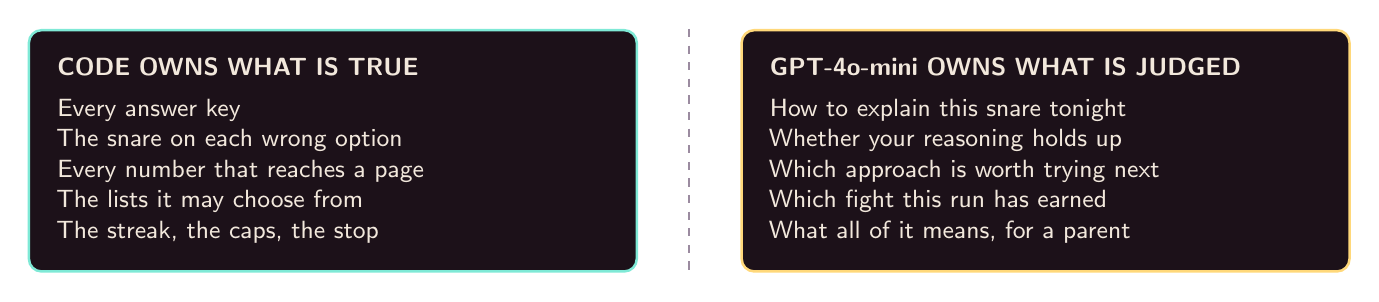
\begin{tikzpicture}
  \node[cool, text width=70mm, align=left, minimum height=0mm, inner sep=3.6mm] (L)
    {\textbf{CODE OWNS WHAT IS TRUE}\\[0.4em]
     Every answer key\\
     The snare on each wrong option\\
     Every number that reaches a page\\
     The lists it may choose from\\
     The streak, the caps, the stop};
  \node[gld, text width=70mm, align=left, minimum height=0mm, inner sep=3.6mm,
        right=13mm of L] (R)
    {\textbf{\themodel\ OWNS WHAT IS JUDGED}\\[0.4em]
     How to explain this snare tonight\\
     Whether your reasoning holds up\\
     Which approach is worth trying next\\
     Which fight this run has earned\\
     What all of it means, for a parent};
  \draw[Muted, line width=0.9pt, dashed]
    ($(L.north east)!0.5!(R.north west)$) -- ($(L.south east)!0.5!(R.south west)$);
\end{tikzpicture}
\end{adjustbox}
\end{center}

\vspace{0.2em}
Every one of those left-hand rows is there because we watched the right-hand
side get something wrong first. Four shields came out of that.

\begin{shieldbox}
\textbf{Shield 1 --- \themodel\ never redoes the maths.}\\
Asked to re-explain a question it had already solved, it would quietly redo the
sums and land somewhere new, in confident prose, right next to the correct
answer. So the verified working now rides inside the prompt as the only
arithmetic it is allowed to state. Its job is to explain \emph{why} your method
fails, never to recompute.
\end{shieldbox}

\begin{shieldbox}
\textbf{Shield 2 --- the snare is read, not guessed.}\\
Every wrong option in the vault carries the faulty thinking that produces it.
When you pick one, the game looks the snare up. No model call, no inference, no
chance of naming the wrong trap and teaching you a lesson you did not need.
\end{shieldbox}

\begin{shieldbox}
\textbf{Shield 3 --- a written question must survive itself.}\\
We caught the model writing a perfectly good question and marking the wrong
option as the answer. A student would have been told they were wrong for being
right. So now anything \themodel\ writes has to solve itself again \emph{blind}
--- without seeing the key it just wrote --- and the two answers have to match.
They disagree, the question is destroyed and nobody ever sees it.
\end{shieldbox}

\vspace{0.4em}
\begin{center}
\begin{adjustbox}{max width=\textwidth}
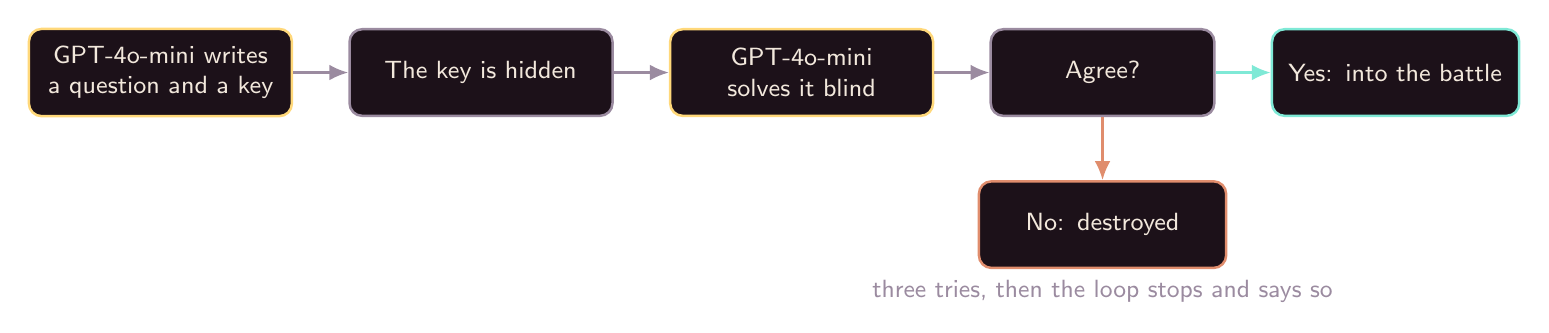
\begin{tikzpicture}[node distance=7mm]
  \node[gld] (write) {\themodel\ writes a question and a key};
  \node[box, right=of write] (hide) {The key is hidden};
  \node[gld, right=of hide] (solve) {\themodel\ solves it blind};
  \node[box, right=of solve, text width=24mm] (match) {Agree?};
  \node[cool, right=of match, text width=27mm] (show) {Yes: into the battle};
  \node[hot, below=8mm of match, text width=27mm] (bin) {No: destroyed};
  \draw[arrow] (write)--(hide);
  \draw[arrow] (hide)--(solve);
  \draw[arrow] (solve)--(match);
  \draw[arrowcool] (match)--(show);
  \draw[arrowhot] (match)--(bin);
  \node[tag, below=1mm of bin] {three tries, then the loop stops and says so};
\end{tikzpicture}
\end{adjustbox}
\end{center}

\begin{shieldbox}
\textbf{Shield 4 --- \themodel\ may not put a number on the page.}\\
It once wrote ``beaten three tricks'' when one had been beaten, borrowing a 3
that belonged to a different count on the same screen. Checking figures one at
a time cannot catch a real number attached to the wrong noun. So the rule is
absolute: on the page that goes to a parent, code prints every figure and
\themodel\ prints none. Any reply containing a number --- in digits or spelled
out --- is thrown away and a sentence built from the same facts goes out
instead.
\end{shieldbox}

\vspace{0.3em}
There is a fifth guard that is not about the model at all. In an early draft of
the vault, 58\% of the correct answers sat on option A. A player who always
guessed A would have scored well and learnt nothing. The key is now balanced
across all four letters, and every note about a wrong answer is keyed to the
answer's \emph{text}, so it stays true however the options are shuffled.

\begin{quietbox}
Underneath all of it, one sentence: \textbf{a small model is a capable judge and
an unreliable authority.} Everything \themodel\ says in this game is a
judgement. Nothing it says is the source of what is mathematically true.
\end{quietbox}

% =====================================================================
\section{When the snare holds}

Some nights you do not beat it. The game has a rule for this, and it is
deliberately not \themodel's to bend: after four fresh questions, or after all
four ways of explaining have been tried, or once the model has been called as
many times as its budget allows, the training stops. It does not keep drilling
you into the ground. It tells you the battle is ending, and \emph{why} it is
ending, and it says plainly that a real person is probably more use to you now
than one more question from a computer. A note goes home naming every approach
that was already tried, so whoever helps you next does not start from scratch.

That is also the moment the Collector notices you. He is the giant skull that
hangs above the whole citadel, and the five monsters are afraid of him --- from
your very first battle they whisper warnings that something older is watching.
He is what those warnings meant. He does not set new snares or teach anything.
He goes after the arithmetic you are supposed to already own --- the quick
sums a snare can hide behind when you are slow with them --- and he goes after
it against a clock: \textbf{ten questions, eight seconds each, three lives}.
This is speed, not curriculum, so nothing that happens in his arena counts
against your quiz record. You cannot make things worse by facing him. You can
only get faster.

\shot{collector.png}{The Collector's speed trial: ten questions, eight seconds
each, three lives. Nothing here counts against your record --- it is pure
speed.}

Lose to him --- and most people will, the first time --- and he sends you down
to one of his three lieutenants. Each lieutenant is a smaller, faster fight
built around a single mental shortcut: not a topic from the course, but a trick
of arithmetic that makes the whole thing quicker once it is automatic. The
Collector is fast because these shortcuts are second nature to him. The
lieutenants are where you make them second nature too.

\vspace{0.4em}
\begin{center}
\begin{tabularx}{0.97\textwidth}{@{}>{\sffamily\bfseries\color{Coral}}l X@{}}
\toprule
Twinfang & Doubling and halving. Double by adding a number to itself; multiply
by 4 by doubling twice.\\
\addlinespace[0.25em]
The Niner & Nines, fast. Multiply by 10, then subtract the number once.\\
\addlinespace[0.25em]
Splitjaw & Making tens. $47+38$ becomes $47+3$, then $+35$.\\
\bottomrule
\end{tabularx}
\end{center}
\vspace{0.4em}

Each drill is a burst: ninety seconds, three lives, a stream of quick sums of
that one kind. Before you step in, \themodel\ leans over and whispers the
shortcut in a sentence or two --- not the full lesson, just the move --- so you
go in armed rather than guessing. When the ninety seconds are up it reads the
exact questions you got wrong, names the one pattern running through them, and
gives you a few more of that precise kind to try. It is the same teach-and-check
idea as the main battles, shrunk down to raw speed.

And it decides where you go next the same way it decides everything else ---
from evidence, not a guess. It looks at which lieutenants you have actually
fought and how you scored against each, and points you at the one that will
help most, saying out loud why it chose that one. Beat the lieutenants, get
faster, and go back up to try the Collector again. You keep everything you have
already won; a bad run against him takes nothing away.

Retreating from any fight is free. The monsters remember it, and they will
mention it when you come back.

% =====================================================================
\section{A letter reaches home}

After a battle, a note is written for whoever is at home. Not only on the bad
nights --- a parent who only hears from us on the worst day cannot see a
pattern, so notes go after any battle with mistakes in it, after a hand-off,
and after a win.

The note says which monster was fought, which snare caught you most, which
explanations were tried, whether the snare fell or is still standing, and three
things to try at the kitchen table with coins, cups, food or paper. Ten
minutes, no jargon, nothing to buy. And it is about one evening --- it is not a
label anyone gets to keep.

\shot{letters.png}{The page a parent sees. Every figure on it is placed by
code; \themodel\ only turns those facts into a note a family can act on.}

One button on that page prints a practice sheet: up to ten questions on that
one snare, room to write under each, and the answer key on its own page so a
parent can hand over the questions without handing over the answers. Vault
questions first, because those come with working a parent can check. Anything
\themodel\ writes to fill the sheet has already solved itself blind, the same as
on screen. If it cannot fill ten, the sheet comes out short. It never comes out
with a question we could not verify.

% =====================================================================
\section{It really runs, deployed online}

\begin{center}
\begin{adjustbox}{max width=\textwidth}
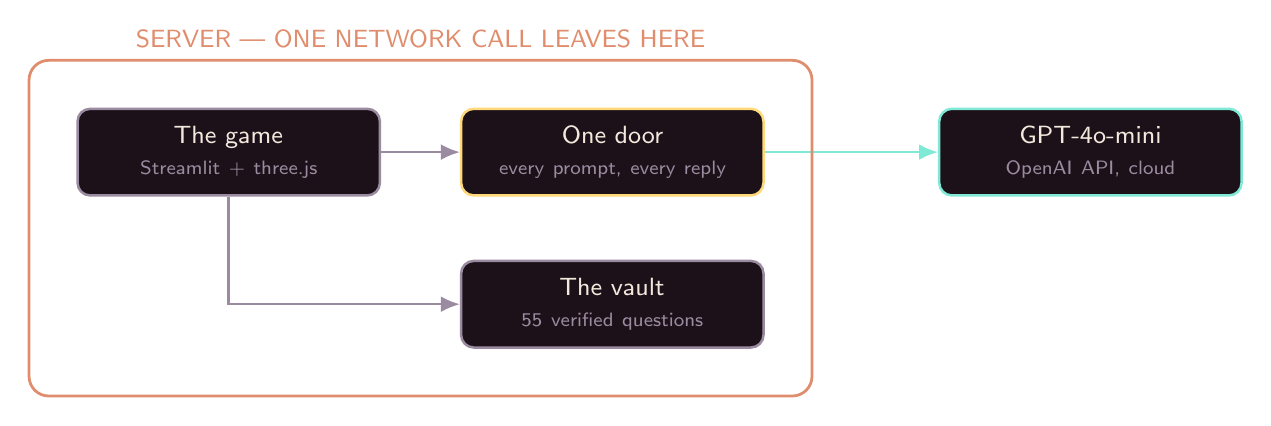
\begin{tikzpicture}[node distance=6mm]
  \node[box, text width=34mm] (ui) {The game\\{\scriptsize\color{Muted}Streamlit + three.js}};
  \node[gld, right=10mm of ui, text width=34mm] (door) {One door\\{\scriptsize\color{Muted}every prompt, every reply}};
  \node[box, below=8mm of door, text width=34mm] (vault) {The vault\\{\scriptsize\color{Muted}55 verified questions}};
  \node[cool, right=22mm of door, text width=34mm] (model) {\themodel\\{\scriptsize\color{Muted}OpenAI API, cloud}};
  \draw[arrow] (ui)--(door);
  \draw[arrowcool] (door)--(model);
  \draw[arrow] (ui.south) |- (vault.west);
  \node[draw=Coral, line width=1pt, rounded corners=2.5mm,
        fit=(ui)(door)(vault), inner sep=6mm] (server) {};
  \node[tag, text=Coral, above=1mm of server.north] {SERVER --- ONE NETWORK CALL LEAVES HERE};
\end{tikzpicture}
\end{adjustbox}
\end{center}

\vspace{0.3em}
The whole game exists and you can play it end to end today: the opening scene,
the citadel you can orbit, five monster halls, the training loop, the Collector
and his three lieutenants, the notes home and the printable sheets, and the
gate that opens when the last seal breaks.

No account, no sign-in. Three.js is still vendored into the repository, the
monster models are still CC0, the audio is still ours --- none of the game's
own assets are pulled from a CDN. But this is no longer an offline claim: an
internet connection is required to play, because every \themodel\ call ---
the lesson, the hint, the reasoning judgement, the letter home --- travels to
OpenAI's servers and back. A fourteen-year-old's typed answer and their typed
reasoning are part of that traffic. That trade-off bought something real: the
game runs anywhere a browser can reach it, with no local model to install and
no laptop-class GPU required to serve it. It also means the strongest privacy
claim this brief could once make --- that nothing a student writes leaves the
machine --- no longer holds, and should not be repeated in front of judges.

And if \themodel's API key is missing or a call fails, the app still opens,
still runs the quiz, still marks it, and says plainly where the writing would
have been.

% =====================================================================
\vfill
{\color{Muted}\hrule height 0.4pt}
\vspace{0.6em}
\begin{center}
{\sffamily\small\bfseries\color{Coral}Gokulakrishnan $\cdot$ Padmanabha $\cdot$
Taha $\cdot$ Naimah $\cdot$ Amarah}\\[0.3em]
{\small\color{Muted}Originally built for Build with AI --- Gemma Hackathon
$\cdot$ GDG Windsor $\cdot$ Edge / On-Device --- track claim now under review}
\end{center}

\end{document}
